\documentclass[../main.tex]{subfiles}

\begin{document}

\problem{2}

A one-dimensional, \textit{second order} element is shown below:

\begin{figure}[h!]
    \centering
    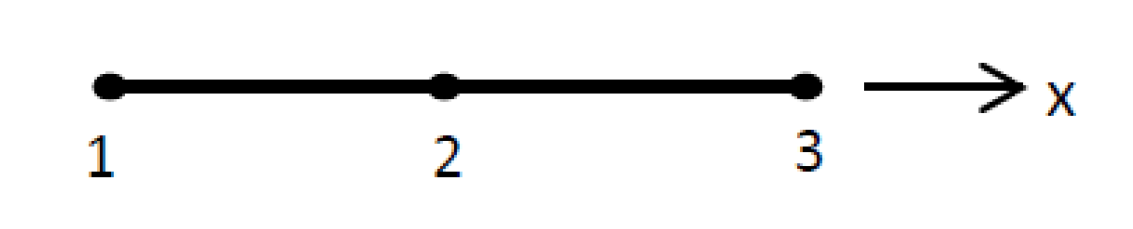
\includegraphics[scale=0.4]{../../images/problem_2/1D_element}
\end{figure}

The physical node locations and nodal displacement values are shown in table \ref{1D_el}:

\begin{table}[h!]
    \centering
    \begin{tabular}{|c|c|c|c|c|c|}
    \hline
    \multicolumn{2}{|c|}{\textbf{Node 1}} & \multicolumn{2}{c|}{\textbf{Node 2}} & \multicolumn{2}{l|}{\textbf{Node 3}} \\ \hline
    \(x_1\) & \(d_1\) & \(x_2\) & \(d_2\) & \(x_3\) & \(d_3\) \\ \hline
    2 in. & 0.15 in. & 4 in. & 0.05 in. & 6 in. & -0.10 in. \\\hline
    \end{tabular}
    \caption{1D element coordinates and displacements.}
    \label{1D_el}
\end{table}

Find the physical location (\(x=\)) on the element where the displacement is zero.

\solution{}

\[
    u = a_1 + a_2x + a_3x^2
\]

\[
    \begin{Bmatrix}
        u_1 \\ u_2 \\u_3
    \end{Bmatrix}
     = [A]
     \begin{Bmatrix}
        1 \\ x \\x^2
    \end{Bmatrix}
\]

\[
    A = \mqty[
        1 & x_1 & x_1^2\\
        1 & x_2 & x_2^2\\
        1 & x_3 & x_3^2
    ]
    =
    \mqty[
        1 & 2 & 4\\
        1 & 4 & 16 \\
        1 & 6 & 36
    ]
\]

\[
    [N] = \mqty[1 & x & x^2][A]^{-1}
\]

\[
    [A]^{-1} = 
    \mqty[
        3 & -3 & 1\\
        -\frac{5}{4} & 2 & \frac{3}{4}\\
        \frac{1}{8} & -\frac{1}{4} & \frac{1}{8}
    ]
\]

\[
    \mqty[N_1 & N_2 & N_3] = \mqty[1 & x & x^2] \mqty[
        3 & -3 & 1\\
        -\frac{5}{4} & 2 & \frac{3}{4}\\
        \frac{1}{8} & -\frac{1}{4} & \frac{1}{8}
    ]
\]

\[
    \mqty[N_1 & N_2 & N_3] = \mqty[\left({\frac{x^2}{8}-\frac{5x}{4}+ 3}\right) & \left({-\frac{x^2}{4}+2x-3}\right) & \left({\frac{x^2}{8}-\frac{3x}{4}+1}\right)]
\]

\[
    \{u\} = [N]\{d\}
\]

\[
    u =  \mqty[\left({\frac{x^2}{8}-\frac{5x}{4}+ 3}\right) & \left({-\frac{x^2}{4}+2x-3}\right) & \left({\frac{x^2}{8}-\frac{3x}{4}+1}\right)] 
    \begin{Bmatrix}
        0.15 \\ 0.05 \\ -0.10
    \end{Bmatrix}
\]

\[
    u = -\frac{x^2}{160} - \frac{x}{80} + \frac{1}{5}
\]

\[
    \boxed{
    u(x=4.7445) = 0
    }
\]

\begin{figure}[h!]
    \centering
    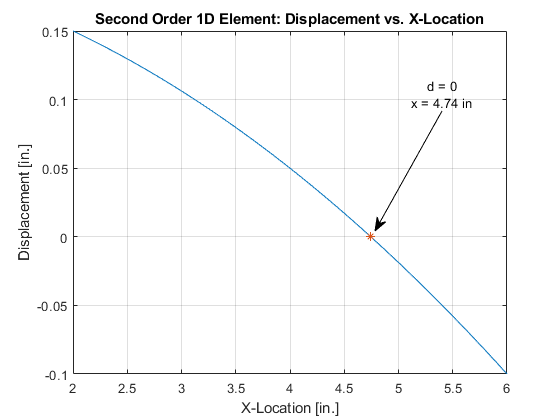
\includegraphics[scale=1]{../../images/problem_2/deflection_plot.png}
    \caption{Deflection vs. X-location for second order 1D element. Zero deflection point starred in red.}
    \label{deflection_plot}
\end{figure}

\end{document}